\chapter{Dise\~no e implementaci\'on de la soluci\'on}
\label{cap:diseno}

Esta etapa contempla el diseño de la solución correspondiente a un algoritmo memético (\textbf{MA}) para predecir la estructura terciaria de la proteína.

\section{Algoritmo memético para el problema 3-D PSP}

Como se revisó en la sección \ref{fundamentos:memeticos}, los algoritmos meméticos son algoritmos evolutivos que aprovechan toda la información disponible para mejorar los agentes de la población, de forma activa mediante el uso de búsqueda local.

También, el enfoque que adopta el MA es el visto en la sección \ref{fundamentos:abinitio-db}, ya que se usará la función de energía potencial \textit{Amber Force Field 14 SB} (versión actualizada de \textit{Amber Force Field 99 SB}, \citealp{amber14}) como función de minimización. El conocimiento biológico que usa el MA para generar sus agentes y modificarlos, viene dado por lo observado experimentalmente en la naturaleza, esta información está almacenada en la \textit{Protein Data Bank}. 
 
Para hacer uso de esta información a nivel algorítmico se debe crear una estructura que indique cuáles son los ángulos más probables para un aminoácido según la estructura secundaria en la que se encuentra. Por ejemplo, si el residuo Alanina está dentro de una $\alpha$-helix, el método debe escoger con una alta probabilidad los ángulos de torsión que más usa este residuo para formar dicho estado conformacional. Para realizar esta elección de ángulos se usará la \textit{Lista de ángulos de probabilidades de ocurrencia \textbf{APL}} desarrollada en \citealp{Dorn:2013} y que está explicada a continuación.

\subsection{Lista de ángulos de probabilidades de ocurrencia APL}
Este algoritmo toma ventaja del conocimiento experimental almacenado en la Protein Data Bank (\citealp{Berman:2000}). Los pares de ángulos $\phi$ y $\psi$ pueden tomar valores reales entre $-180º$ y $180º$. En consecuencia, el espacio de búsqueda por cada residuo es astronómicamente amplio y la complejidad del problema aumenta según se incremente la cantidad de residuos. No obstante, si se visualiza la información almacenada en la PDB se ve que los diferentes residuos tienen diferentes distribución de ángulos. En la figura \ref{fig:rmc-glicina} se puede observar que los pares de ángulos más usados están en dos regiones representadas por el área de color más oscuro.

\begin{figure}[H]
	\centering
	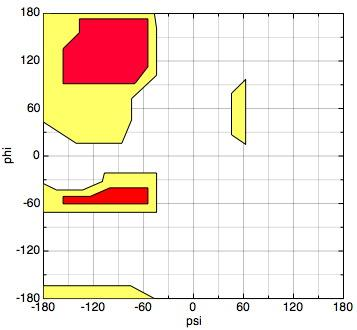
\includegraphics[scale=.5]{images/rama-plot.jpg}
	\caption{\em Ejemplo de mapa de Ramachandran para los ángulos \textphi~y~\textpsi~de un amino\'acido (pág. 105 \citealp{book:kessel}).}
	\label{fig:rmc-glicina} 
\end{figure}

La gran ventaja de incorporar esta información al algoritmo memético es poder reducir el espacio de búsqueda de soluciones, mediante la asignación de probabilidades de selección de ángulos según su ocurrencia experimental.

Para incluir esta información se construirá un histograma \textit{$H_{a,z}$} de $361{\times}361$ celdas para cada residuo de aminoácidos \textit{a} con estructura secundaria \textit{z}. Cada celda $(i,j)$ tendrá el número de veces que el par \textit{(a,z)} ha tenido esa coordenada presente. En orden de incrementar la representación de las áreas más densas, los valores de las 8 celdas adyacentes a $(i,j)$ serán tomadas en consideración, ver fórmula \ref{eq:histogram}. 

\begin{equation}
	\label{eq:histogram}
	H'_{a,z}(i,j)=\sum_{r=i-1}^{i+1}\sum_{s=j-1}^{j+1}H_{a,z}(r,s)
\end{equation}
\\[15pt]
Luego por cada uno de estos histogramas, se genera una matriz de probabilidad usando la fórmula \ref{eq:apl}.

\begin{equation}
	\label{eq:apl}
	APL_{a,z}(i,j)=\frac{H'_{a,z}(i,j)}{\sum_{\forall x,y}H'_{a,z}(x,y)}
\end{equation}
\\[15pt]
En consecuencia, se deben generar $20_{\text{residuos}} {\times} 8_{\text{e. secundarias}} = 160_{APL}$ que deberán ser cargados al comienzo de la implementación.

\subsection{Estructuras de datos y población}
Todo MA depende de la estructura de su población y de los operadores que se aplicaran para poder alcanzar el objetivo para el cual fueron diseñados. En esta sección se conocerá la estructura de la población, desde cómo se representa una solución dentro de esta hasta las reglas que operan en la población.

\subsubsection{Representación de una Solución}
Cada solución estará representada como el conjunto de 2 tipos de datos.
\begin{itemize}
	\item \textbf{Energía potencial de la solución}: valor tipo flotante.
	\item \textbf{Información de de cada residuo}: arreglo unidimensional del mismo largo \textit{n} de la secuencia de residuos, por cada residuo se guardan 6 valores, 2 para los ángulos $\phi$ y $\psi$ (cadena principal), y 4 para los ángulos $chi_{1}$, $chi_{2}$, $chi_{3}$ y $chi_{4}$ (cadena lateral).
\end{itemize}

\begin{equation*} 
    \begin{split} 
        \text{sol} = \{\text{energía},\text{residuos}\} \\
        \text{residuos} = [[\phi,\psi,\chi_1,\chi_2,\chi_3,\chi_4]_1,...,[\phi,\psi,\chi_1,\chi_2,\chi_3,\chi_4]_n]
    \end{split} 
\end{equation*}

\subsubsection{Concepto de Agente}
La población del algoritmo memético está compuesto por entidades llamadas agentes. Cada agente maneja 2 tipos de soluciones llamadas \textit{Pocket} y \textit{Current}. Las soluciones tipo \textit{Current} son aquellas soluciones que sufren modificaciones mediante los operadores del algoritmo, en palabras simples, estas son las soluciones que evolucionan durante las iteraciones. Las soluciones \textit{Pocket} son la memoria del agente, son aquellas soluciones \textit{Current} que resultaron ser las mejores y han sido guardadas.

\begin{figure}[H]
	\centering
	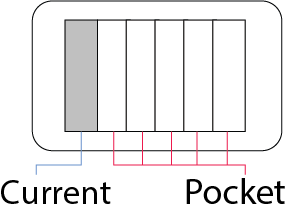
\includegraphics[height=4cm]{images/agent.png}
	\caption{\em Agente de población de MA.}
	\label{fig:agent}
\end{figure}

Los agentes que se usarán en el MA están compuestos por 6 soluciones, 1 \textit{Current} y 5 \textit{Pockets}, es decir, cada agente trabajará con una solución que irá evolucionando y tendrá 5 espacios de memoria reservado para guardar las mejores soluciones encontradas (ver figura \ref{fig:agent}).

\begin{equation*} 
    \begin{split} 
        Agente_i = \{Current, Pockets_{1{\times}5}\}
    \end{split} 
\end{equation*}


\subsubsection{Población}
\label{diseno:poblacion}
La estructura de la población de este método está compuesta por 13 agentes, dispuestos en un árbol ternario en 3 niveles con disposición jerárquica. A medida que se desciende en los niveles, las soluciones son peores, por lo tanto la mejor solución está en la raíz superior del árbol.
Este árbol está dispuesto en subpoblaciones, cada subpoblación contempla dos niveles del árbol, en el nivel superior está el agente líder y en el inferior sus 3 nodos hijos que corresponden a los agentes de apoyo. Cabe notar que los agentes ubicados en el segundo nivel del árbol general son líderes de las subpoblaciones inferiores y agentes de apoyo de la subpoblación superior.

\begin{figure}[tp]
	\centering
	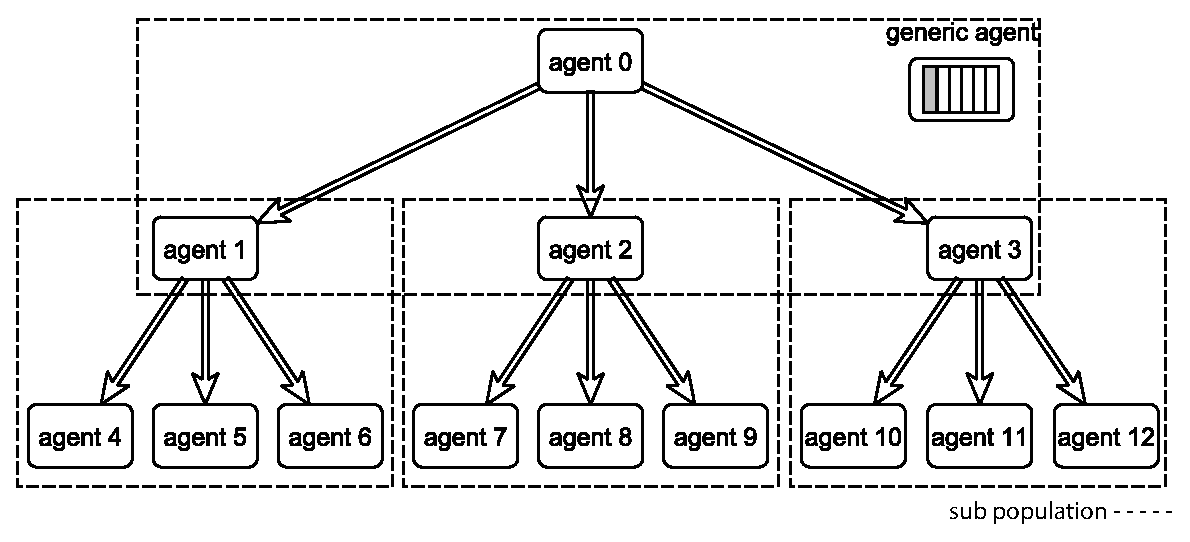
\includegraphics[height=6cm]{images/popStructure.eps}
	\caption{\em Estructura poblacional}
	\label{fig:ternary-pop}
\end{figure}

Tal como se puede ver en la figura \ref{fig:ternary-pop}, existen 4 subpoblaciones que están delimitadas por líneas segmentadas.

\begin{equation*} 
    \begin{split}
        Agente_{n} \text{ es lider de } SubPop_i \Longleftrightarrow n = i ~/~ &i = 0,1,2,3\\
            &n=0,1,\dots,12 \\
        \\    
        Agente_{n} \text{ es soporte de } SubPop_i \Longleftrightarrow n = 3i+j ~/~ &j = 1,2,3\\
        &i=0,1,2,3\\
        &n=0,\dots,12\\
    \end{split} 
\end{equation*}
\\[15pt]


Cada subpoblación tiene dos métodos importantes asociados:
\begin{itemize}
	\item \textbf{Actualización de pockets:} Todos los agentes deben evaluar si guardan la solución \textit{Current} en sus \textit{Pockets}. Esta acción tiene asociada reglas que aplican funciones como $d(A,B)$ que entrega \textit{Verdadero} si las soluciones A y B son diversas y $Energia(A)$ que entrega la energía potencial de la solución A. Con lo mencionado anteriormente, las reglas para realizar una inserción de una solución $S$ en los \textit{Pockets} de un $Agente_i$ son:
        \begin{enumerate}
            \item ($Agente_i$ no está completo) $\wedge$ ($d(S,Pocket^i_j))\geq
            10$), $\forall j$.
             \item ($Agente_i$ no está completo) $\wedge$
            (${\exists}j/d(S,Pocket^{i}_j){<}10$) $\wedge$
            ($Energia(S){<}Energia(Pocket^{i}_{mejor})$). Luego $S$ reemplazará a
            $Pocket^{i}_j$ / $d(S,Pocket^{i}_j))$ es mínima, $\forall j$.
             \item ($Agente_i$ está completo) $\wedge$ ($Energia(S) <
            Energia(Pocket^{i}_{mejor})$).Luego $S$ reemplazará a $Pocket^{i}_j$ /
            $d(S,Pocket^{i}_j))$ es mínima, $\forall j$.
            \item ($Agente_i$ está completo) $\wedge$ ($d(S,Pocket^{i}_j) \geq 10,
            \forall j$) $\wedge$ ($Energia(S) < Energia(Pocket^{i}_{peor})$). Luego $S$
            reemplzará a $Pocket^{i}_{peor}$.
        \end{enumerate}
	\item \textbf{Propagación de pockets:} después de la etapa anterior, el $Pocket_{mejor}$ de los agentes de apoyo es comparado con el $Pocket_{mejor}$ del agente líder de la subpoblación, si la solución del agente de apoyo es mejor que la del líder, se intercambian los pockets.
\end{itemize}

El método \textit{propagación de pockets} se aplica primero en las subpoblaciones inferiores y luego en la subpoblación superior, no al revés.

\subsection{Operadores del algoritmo mem\'etico}
A continuación se muestran los algoritmos de los operadores meméticos a ser implementados.

\subsubsection{Población inicial}

El algoritmo de población inicial se basa en la estructura jerárquica que se puede visualizar en la figura \ref{fig:ternary-pop}. Recibe como entrada la secuencia de aminoácidos que será usada en la predicción y entrega una población con 13 agentes con sus \textit{Currents} inicializados. 

Para ello, cada solución \textit{Current} se crea usando la información almacenada en la APL mediante el llamado a la función $obtenerAngulosDesdeAPL()$ (línea 7, Algoritmo \ref{alg:memetico-initpop}), esta función necesita como entrada el identificador del residuo y la estructura secundaria en la que se encuentra para escoger la APL correspondiente de la que se obtendrán los ángulos $\phi,\psi$. También usa la función $obtenerAngulosChi()$ (línea 9, Algoritmo \ref{alg:memetico-initpop}) para inicializar los valores de los ángulos de la cadena lateral, estos son provistos por la biblioteca Dunbrack (\citealp{dunbrack}) . Una vez que todos los residuos de la solución están completos, se calcula la energía de la solución (línea 12, Algoritmo \ref{alg:memetico-initpop}). Finalmente, se guarda la solución en el Current, este proceso se repite por cada agente de la población.
\\[25pt]
\begin{algorithm}[H]
	\begin{algorithmic}[1]
		\REQUIRE $secuencia$: secuencia de residuos
		\ENSURE $pop$: población de agentes
		\STATE $pop \leftarrow \textbf{popVacia}()$
		\FOR {$i=0:12$}
		    \STATE $pop[i] \leftarrow \textbf{agenteVacio}()$
			\STATE $sol \leftarrow \textbf{solVacia}()$
			\FOR {\textbf{each} residuo \textbf{in} $secuencia$}
				%\STATE $resid \leftarrow \textbf{obtenerAminoNumID}(residuo)$
				%\STATE $secundid \leftarrow \textbf{obtenerEstructuraSecundariaID}(residuo, secuencia)$
				\STATE \COMMENT ángulos $\phi$ y $\psi$ de la cadena principal
				\STATE $\phi,\psi \leftarrow \textbf{obtenerAngulosDesdeAPL}(sol, residuo, estruc)$
				%\STATE $\phi' \leftarrow \phi + random(-1,1)$
				%\STATE $\psi' \leftarrow \psi + random(-1,1)$
				\STATE \COMMENT ángulos $\chi$  de la cadena lateral
				\STATE $\chi_{angulos} \gets \textbf{obtenerAngulosChi}(residuo)$
				\STATE $sol.residuo[j] \leftarrow \phi,\psi,\chi_{angulos}$
			\ENDFOR
			\STATE $sol.energia \gets \textbf{calcularEnergia}(sol) $
			\STATE $pop[i].current \leftarrow sol$
		\ENDFOR
		\RETURN $pop$
	\end{algorithmic}
	\caption{Algoritmo Población Inicial}
	\label{alg:memetico-initpop}
\end{algorithm}

\subsubsection{Cruzamiento}
El algoritmo de cruzamiento tiene como fin otorgar la característica evolutiva al algorítmo memético, ya que mediante la reproducción se puede conservar características de las mejores soluciones a la vez que se diversifica la población, con la incorporación de las soluciones descendientes.

Respecto al funcionamiento, requiere dos soluciones A y B, que serán las soluciones que se cruzarán (Entrada de Algoritmo \ref{alg:memetico-cruzamiento}). Para generar la nueva solución, se crea una solución vacía y cada uno de sus residuos serán tomados del padre A o del padre B, para esta decisión se utiliza la función \textit{seleccionarDesdePadreA()} (línea 4, Algoritmo \ref{alg:memetico-cruzamiento}), si es verdadero se guardará la información del residuo del padre A en la nueva solución, de lo contrario, se tomará la información del residuo del padre B.
\\[25pt]
\begin{algorithm}[H]
	\begin{algorithmic}[1]
		\REQUIRE $sol_{A}$ y $sol_{B}$: soluciones a ser cruzadas
		\ENSURE \textit{descendiente}: nueva solución
		\STATE \textit{descendiente} $\leftarrow solVacia()$
		\FOR{$i=1:largoSecuencia$}
			\IF{$\textbf{hacerCruzamiento}()$}
    			\IF{$\textbf{seleccionarDesdePadreA}()$}
    				\STATE \textit{descendiente}.\textit{residuo}[i] $\gets sol_{A}.residuo[i]$
    			\ELSE
    				\STATE \textit{descendiente}.\textit{residuo}[i] $\gets sol_{B}.residuo[i]$
    			\ENDIF
			\ENDIF
		\ENDFOR
		\STATE \textit{descendiente.energia} $\gets \textbf{calcularEnergia}(descendiente)$
		\RETURN \textit{descendiente}
	\end{algorithmic}
	\caption{Algoritmo de Cruzamiento}
	\label{alg:memetico-cruzamiento}
\end{algorithm}

\subsubsection{Búsqueda local: \textit{Simulated annealing} con saltos de búsqueda}

Anteriormente se explicó la diferencia entre un individuo y un agente, se recalcó que un agente es un ente activo, esta actividad se ve reflejada en la capacidad de mejorar a lo largo del tiempo de manera conducida, para ello los agentes hacen uso de la búsqueda local que usa información característica del problema. En este trabajo se hace una adaptación del algoritmo de \textit{Enfriamiento Simulado (Simulated Annealing SA, \citealp{Kirkpatrick1983})} que implica la posibilidad de cambiar el punto de origen de la búsqueda.

\begin{figure}[tp]
	\centering
	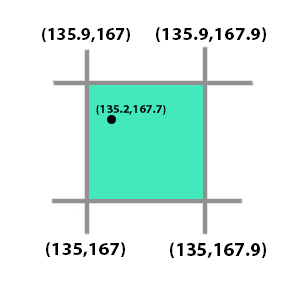
\includegraphics[scale=.7]{images/ls-range.jpg}
	\caption{\em Ejemplo de rango máximo de alcance del algoritmo de búsqueda local}
	\label{fig:ls-range}
\end{figure}

El algoritmo \ref{alg:localsearch} propone realizar una búsqueda local en la vecindad de los ángulos de cada uno de los residuos de la solución. En primera instancia se evalúa si se mantendrá el punto de origen, si se decide cambiar, la nueva coordenada deberá estar dentro del radio de búsqueda y será escogida usando la función $obtenerAngulosDesdeAPL()$. Luego, se procede a buscar dentro de la vecindad de la coordenada, la función \textit{escogerValorVecino()} buscará ángulos vecinos pero sin salir de la celda de la coordenada. Por ejemplo, si se tiene la coordenada $(135.2,167.7)$, se buscarán ángulos que no salgan de la celda delimitada por $(135.0,167.0)$, $(135.9,167.0)$, $(135.0,167.9)$, $(135.9,167.9)$ tal como se observa en la figura \ref{fig:ls-range}, la vecindad es la zona de color más claro. 
La cantidad de veces que se busca en la vecindad responde a la fórmula \ref{eq:sa-temperature}.
\begin{equation}
    \label{eq:sa-temperature}
    T(t)=T_{\text{inicial}}{\times}\alpha^t
\end{equation}
En donde $T$ es la función de temperatura del SA, $T_{\text{inicial}}$ es la temperatura inicial, $\alpha$ es el factor de enfriamiento y $t$ es el tiempo.

La probabilidad con la que es aceptada una solución es calculada según la ecuación \ref{eq:sa-prob}.

\begin{equation}
    \label{eq:sa-prob}
    P(energia_{mejor},energia_{sol},t) =
    \left\{
        \begin{array}{ll}
            V, & energia_{sol} < energia_{mejor} \\
            V, & exp(\frac{ energia_{mejor}-energia_{sol}}{T(t)}) > random(0,1) \\
            F, & exp(\frac{ energia_{mejor}-energia_{sol}}{T(t)}) \leq random(0,1)
            
        \end{array}
    \right.
\end{equation}
\\[25pt]

\begin{algorithm}[H]
    \begin{algorithmic}[1]
        \REQUIRE $sol$: solución, $salto$: salto máximo permitido 
        \ENSURE $sol$: solución final después de la búsqueda local
        \FOR {\textbf{each} residuo}
            \IF{$\textbf{hacerMejora()}$}
                \IF{$\textbf{cambiarCelda}()$} \label{line:changeAngleCell}
                    \STATE $sol \leftarrow \textbf{obtenerAngulosDesdeAPL}(sol,residuo,estruc,salto)$ \label{line:getAPL}
                    %\STATE $\phi' \leftarrow \phi + random(-1,1)$
                    %\STATE $\psi' \leftarrow \psi + random(-1,1)$
                \ENDIF
                \FOR{\textbf{each} $angulo (\phi,\psi)$ \textbf{in} $sol.residuo[i]$}
                    %\STATE $E_{anterior} \gets sol.energia$
                    %\STATE $energia_{aux} \gets energia_{anterior}$
                    \STATE $t = 0$
                    \REPEAT \label{line:iniSA}
                        %\STATE $sol_{respaldo} \gets sol$
                        \STATE $nuevaSol \gets \textbf{solVecina}(sol.residuo[i], angulo)$
                        \STATE $nuevaSol.energia \gets \textbf{calcularEnergia}(nuevaSol)$
                        \IF{$\textbf{P}(sol.energia,nuevaSol.energia,t)$}
                            \STATE $sol \gets nuevaSol$
                            %\STATE $sol.energia \gets energia_{aux}$
                    %    \ELSE
                    %        \STATE $sol \gets sol_{respaldo}$
                        \ENDIF
                        \STATE $t++$ \COMMENT aumenta la temperatura
                    \UNTIL{$\textbf{T}(t) < 0.1$} \label{line:endSA}
                    %\STATE $sol.energia \gets energia_{aux}$
                \ENDFOR
            \ENDIF
        \ENDFOR
    \RETURN $sol$
    \end{algorithmic}
    \caption{Algoritmo de Búsqueda Local}
    \label{alg:localsearch}
\end{algorithm}


\subsubsection{Mutación}
Con el fin de mantener la diversidad dentro de la población y aumentar la probabilidad de escapar de mínimos locales, se usa el algoritmo \ref{alg:memetico-mutation}. Esto se logra mediante la alteración de los ángulos de la cadena principal. Esta alteración consiste en la adición de un valor entre un intervalo a los ángulos $\phi$ y $\psi$ del residuo que se desea mutar. Cabe mencionar que la aplicación del operador de mutación está sujeto a la probabilidad de mutación ingresada como entrada.
\\[25pt]
\begin{algorithm}[H]
	\begin{algorithmic}[1]
		\REQUIRE$sol$: solución a ser mutada, \\ \hspace{1.2cm} $rango_{mutacion}$: valor que será sumado o restado al ángulo mutado.
		\ENSURE $sol$: solución mutada
		\FOR{$i=1:largoSecuencia$}
    		\IF{$\textbf{siHacerMutacion}()$}
    		    \STATE $sol.residuo[i] \gets sol.residuo[i] + random(-rango_{mutacion}, rango_{mutacion})$
    		\ENDIF
		\ENDFOR
		\STATE $sol.energia \gets \textbf{calcularEnergia}(sol)$
		\RETURN $sol$
	\end{algorithmic}
	\caption{Algoritmo de Mutación}
	\label{alg:memetico-mutation}
\end{algorithm}

\subsubsection{Diversidad}
El operador de diversidad responde si son diversas dos soluciones. Para ello, se basa en la suma de las distancias entre los ángulos de las dos soluciones. Estas distancias son calculadas haciendo uso de la lógica de los mapas de Ramachandran. Los ángulos dihédricos ($\phi$ y $\psi$) toman valores que van de -180$^\circ$ a 180$^\circ$ con la particularidad que -180$^\circ$ es equivalente que 180$^\circ$, por lo tanto, los bordes de los mapas de ramachandran son continuaciones de sus bordes opuestos.

Sea $A$ y $B$ dos soluciones, $D$ la diferencia mínima que debe existir para que dos soluciones sean diferentes, y $D_{A,B}$ la distancia entre $A$ y $B$, y $n$ el largo de la secuencia, la función de diversidad $d$ se define como:

\begin{equation}
    D_{A,B} = \frac{\sum_{i=1}^{n}min(|\Delta(\phi_i,\psi_i)_{A,B}|,360-(|(\phi_i,\psi_i)_{A}|+|(\phi_i,\psi_i)_{B}|))}{n}
\end{equation}

\begin{equation}
    \label{eq:diversity}
    d(S,R) =
    \left\{
        \begin{array}{ll}
            V, & D <  D_{A,B}   \\
            F, & D \geq D_{A,B} \\
        \end{array}
    \right.
\end{equation}
\\[25pt]
\begin{algorithm}[H]
	\begin{algorithmic}[1]
		\REQUIRE $sol_{A}$ y $sol_{B}$: soluciones a ser comparadas. $largoSecuencia$: largo de la secuencia de residuos
		\ENSURE valor de verdad que responde a la compración de las soluciones
		\STATE $diferencia=0$
		\FOR{$i=1:largoSecuencia$}
			\STATE $\phi_{A},\psi_{A} \gets sol_{A}.residuo[i]$
			\STATE $\phi_{B},\psi_{B} \gets sol_{B}.residuo[i]$
			\STATE $diferencia = diferencia + \textbf{min}(|\phi_{A}-\phi_{B}|,360-(|\phi_{A}|+|\phi_{B}|))$
			\STATE $diferencia = diferencia + \textbf{min}(|\psi_{A}-\psi_{B}|,360-(|\psi_{A}|+|\psi_{B}|))$
		\ENDFOR
		\STATE $diferencia = diferencia/largoSecuencia$
		\IF {$diferencia > diversidad$}
		    \RETURN \TRUE
		\ELSE
		    \RETURN \FALSE
		\ENDIF
	\end{algorithmic}
	\caption{Algoritmo de Diversidad}
	\label{alg:memetico-diversidad}
\end{algorithm}

\subsubsection{Actualización de la población}
Tal como se explicó en la sección \ref{diseno:poblacion}, la actualización de la población tiene como función guardar las mejores soluciones y propagar los \textit{pockets} a través de las subpoblaciones de manera ascendente, de forma que, a medida que se sube por el árbol ternario, se encuentren las mejores soluciones.
\\[25pt] 
\begin{algorithm}[H]
	\begin{algorithmic}[1]
		\REQUIRE $pop$: población de agentes
		\ENSURE $pop$: población de agentes ordenadas según estructura jerárquica

		\STATE \COMMENT Primer paso de actualización, guardar currents en pockets
		\FOR{$i=0:12$}
			\STATE $\textbf{reemplazarPeorPocket}(pop[i],pop[i].current)$
		\ENDFOR
		\STATE
		\STATE \COMMENT Segundo paso, propagar mejores pockets en las subpoblaciones inferiores
		\FOR{$i=1:3$}
			\STATE $x_{agente},y_{pocket} \gets \textbf{escogerMejorPocket}(pop[3i+1],pop[3i+2],pop[3i+3])$
			\IF{$pop[x_{agente}].pocket[y_{pocket}] < pop[i].pocket[0].energia$}
				\STATE $\textbf{intercambiarPockets}( pop[i].pocket[0], pop[x_{agente}].pocket[y_{pocket}])$
			\ENDIF
		\ENDFOR
		\STATE
		\STATE \COMMENT Tercer paso, propagar mejor pocket de la subpoblación superior
		\STATE $x_{agente},y_{pocket} \gets \textbf{escogerMejorPocket}(pop[1],pop[2],pop[3])$
		\IF{$pop[x_{agente}].pocket[y_{pocket}] < pop[0].pocket[0].energia$}
			\STATE $\textbf{intercambiarPockets}( pop[0].pocket[0], pop[x_{agente}].pocket[y_{pocket}])$
		\ENDIF
		
		\RETURN $pop$
	\end{algorithmic}
	\caption{Algoritmo de Actualización de la población}
	\label{alg:memetico-updatepop}
\end{algorithm}

\subsubsection{Reinicio}
El algoritmo de reinicio tiene como finalidad hacer escapar de la convergencia al algoritmo memético, reinicializando los \textit{currents} usando el operador APL y eliminando los 4 peores \textit{pockets} de todos los Agentes. Además, el algoritmo memético final incorpora un control de reinicio variable, es decir, toma en consideración la cantidad de generaciones que se necesitaron para converger, dicho tiempo lo considera como nueva cantidad máxima de generaciones sin mejora para realizar el próximo reinicio.
\\[25pt]
\begin{algorithm}[H]
	\begin{algorithmic}[1]
		\REQUIRE $pop$: población de agentes
		\ENSURE $pop$: población de agentes reiniciada
		\FOR{$i=0:12$}
			\STATE $pop[i].current\gets \textbf{nuevaSolucionAleatoria}()$
			\STATE \COMMENT se conserva $pop[i].pocket[0]$
			\STATE $pop[i].pocket[1] \gets \textbf{solVacia}()$
			\STATE $pop[i].pocket[2] \gets \textbf{solVacia}()$
			\STATE $pop[i].pocket[3] \gets \textbf{solVacia}()$
			\STATE $pop[i].pocket[4] \gets \textbf{solVacia}()$
		\ENDFOR
		\RETURN $pop$
	\end{algorithmic}
	\caption{Algoritmo de Reinicio}
	\label{alg:memetico-restart}
\end{algorithm}

\section{Algoritmo memético final}
Tras las explicaciones de los algoritmos y operadores principales que se usarán en la implementación final, se procede a la adaptación del algoritmo memético general para obtener el algoritmo principal (ver algoritmo \ref{alg:memetico-final}) que da solución al problema 3-D PSP.

Este algoritmo memético contempla como entrada la cantidad máxima de tiempo de ejecución medida en segundos, el número máximo de generaciones sin mejora para reiniciar la población del memético, y la estructura primaria y secundaria de la proteína.

Siguiendo al algoritmo general, se comienza haciendo uso del algoritmo de poblado inicial. Una vez inicializado cada \textit{current} de los 13 agentes, se realiza la actualización de la población para empezar a guardar y propagar los pockets de los agentes. Luego, en cada generación se realizará el cruzamiento de la subpoblación superior, esto significa que los \textit{currents} de los Agentes de apoyo serán poblados con el resultado del cruzamiento entre la solución guardada en el \textit{pocket[0]} del $Agente_0$ y el \textit{pocket[0]} de los \textit{Agentes de apoyo} respectivamente. Para terminar la etapa de cruzamiento se realiza el mismo procedimiento pero con las 3 subpoblaciones inferiores. Posteriormente, se busca mejorar los \textit{currents} mediante la aplicación del algoritmo de búsqueda local que hará uso del radio de salto, este radio irá disminuyendo a medida que pasan las generaciones, cuando el radio de búsqueda sea menor a 1 significa que no se podrán realizar más saltos. Finalmente se aplica el operador de mutación y se evalúa si el algoritmo debe reiniciar la población, para detectar si se debe realizar el reinicio se usa la cantidad de generaciones que la población no ha presentado mejoras, si este valor llega al máximo valor permitido (que ingresa como parámetro de entrada al algoritmo), se reinicia la población.
\\[25pt]
\begin{algorithm}[H]
    \begin{algorithmic}[1]
        \REQUIRE $tiempo_{max}$: tiempo de ejecución del MA, $secuencia$: secuencia de aminoácidos
        \ENSURE $sol_{mejor}$: mejor solución encontrada
%        \STATE $tiempo_{inicial} \gets obtenerTiempoActual()$
        \STATE \textit{//generación de población inicial aleatoria}
        \STATE $pop \gets \textbf{pobInicial}(secuencia)$
        \STATE $pop \gets \textbf{actualizarPob}(pop)$
        \STATE $sol_{mejor} \gets pop[0].pocket[0]; gen \gets 0$
        \STATE $contador \gets 0$; $radio \gets 90$
        \REPEAT
            \STATE \textit{//Selección y cruzamiento}
            \FOR{\textbf{each} agente$_i$, $i=1:12$}
            \STATE $padre_1 =
pop[\lfloor(i-1)/3\rfloor].pocket[random(1:5)]$ \label{line:par1}
            \STATE $padre_2 = pop[i].pocket[random(1:5)]$; \label{line:par2}
        \STATE $pop[i].cur \gets
\textbf{crossover}(pop[\lfloor(i-1)/3\rfloor].pocket[padre_1], pop[i].pocket[padre_2])$
            \STATE $pop[i].cur \gets \textbf{crossover}(padre_1,padre_2)$
\label{line:crossover}
            \ENDFOR
            \STATE \textit{//Búsqueda local y mutación}
            \FOR{$i=1:12$}
                \STATE $pop[i].cur \gets
\textbf{busquedaLocalSA}(pop[i].cur,radio)$
                \STATE $pop[i].cur \gets \textbf{mutacion}(pop[i].cur)$
            \ENDFOR
            \STATE $radio = 0.85{\times}radio$
            \STATE $pop \gets \textbf{actualizarPob}(pop)$
\textit{//Control de reinicio}
            \IF{$sol_{mejor} >= pop[0].pocket[0]$}
                \STATE $contador++$
            \ELSE
                \STATE $contador \gets 0$
                \STATE $sol_{mejor} \gets pop[0].pocket[0]$
            \ENDIF
            \IF{$contador == genSinMejora$}
                \STATE $pop \gets \textbf{reiniciarPob}(pop)$
\label{line:restart}
                \STATE $radio \gets 90$; $contador \gets 0$
                \STATE $genSinMejora \gets (gen-ultimoReinicio)$
                \STATE $ultimoReinicio \gets gen$
            \ENDIF
            \STATE $gen \gets gen + 1$
        \UNTIL $tiempo_{max}$
        \RETURN $sol_{mejor}$
        \end{algorithmic}
        \caption{Algoritmo memético final}
		\label{alg:memetico-final}
\end{algorithm}
